\section{Αναπαράσταση Λέξεων σε Διανύσματα}
Για να γίνει δυνατή η επεξεργασία της φυσικής γλώσσας από νευρωνικά δίκτυα πρέπει πρώτα κάθε λέξη να αποκτήσει μορφή η οποία μπορεί να επεξεργαστεί από αυτά. Οι λέξεις μετατρέπονται σε διανύσματα, τα οποία ονομάζονται \emph{word embeddings}.

\subsection{Δημιουργία Λεξιλογίου/Συμβολισμού}
Η δημιουργία λεξιλογίου, \emph{tokenization}, είναι μία διαδικασία διαχωρισμού κειμένου σε μικρότερα κομμάτια που ονομάζονται σύμβολα (\emph{tokens}). Τα σύμβολα του λεξιλογίου μπορεί να είναι ή ολόκληρες λέξεις (\emph{word tokenization}) ή χαρακτήρες (\emph{character tokenization}) ή υπό-λέξεις (\emph{n-gram tokenization}, όπου n ο αριθμός των \emph{tokens} που μπορούν να συνδυαστούν για την παραγωγή μιας λέξης). Συνήθως τα μοντέλα επεξεργασίας φυσικής γλώσσας χρησιμοποιούν λεξιλόγια που χρησιμοποιούν συνδυασμό των παραπάνω τεχνικών για την κάλυψη μεγάλου εύρους της φυσικής γλώσσας. Μέσω του λεξιλογίου μπορεί να παραχθεί, όπως παρουσιάζεται στη συνέχεια, μία αντιστοίχηση της φυσικής γλώσσας σε αριθμητικά διανύσματα τα οποία μπορούν στη συνέχεια να επεξεργαστούν από νευρωνικά δίκτυα. 

\subsection{One-hot Encoding}
Η \emph{one-hot encoding} αποτελεί από τις πιο απλές αναπαραστάσεις προτάσεων σε διάνυσμα. Κάθε πρόταση αναπαρίσταται από ένα διάνυσμα με διάσταση όσο και το μέγεθος του λεξιλογίου. Το λεξιλόγιο είναι το σύνολο με κάθε πιθανή λέξη  που μπορεί να εμφανιστεί σε μία πρόταση. Κάθε θέση στο διάνυσμα αντιστοιχεί σε μία λέξη του λεξιλογίου. Έτσι αν μία λέξη εμφανίζεται στη πρόταση εισόδου τότε η αντίστοιχη τιμή στο διάνυσμα τίθεται $1$ διαφορετικά $0$, \autoref{fig:vector}.

\subsection{Bag of Words/Count Encoding}
Η τεχνική \emph{bag of words} ακολουθεί την ίδια διαδικασία δημιουργίας του διανύσματος με τη διαφορά ότι κάθε κελί του διανύσματος δείχνει τη συχνότητα εμφάνισης της αντίστοιχης λέξης του λεξιλογίου, \autoref{fig:vector}.

\begin{figure}[!ht]
  \centering
  \captionsetup{justification=centering}
  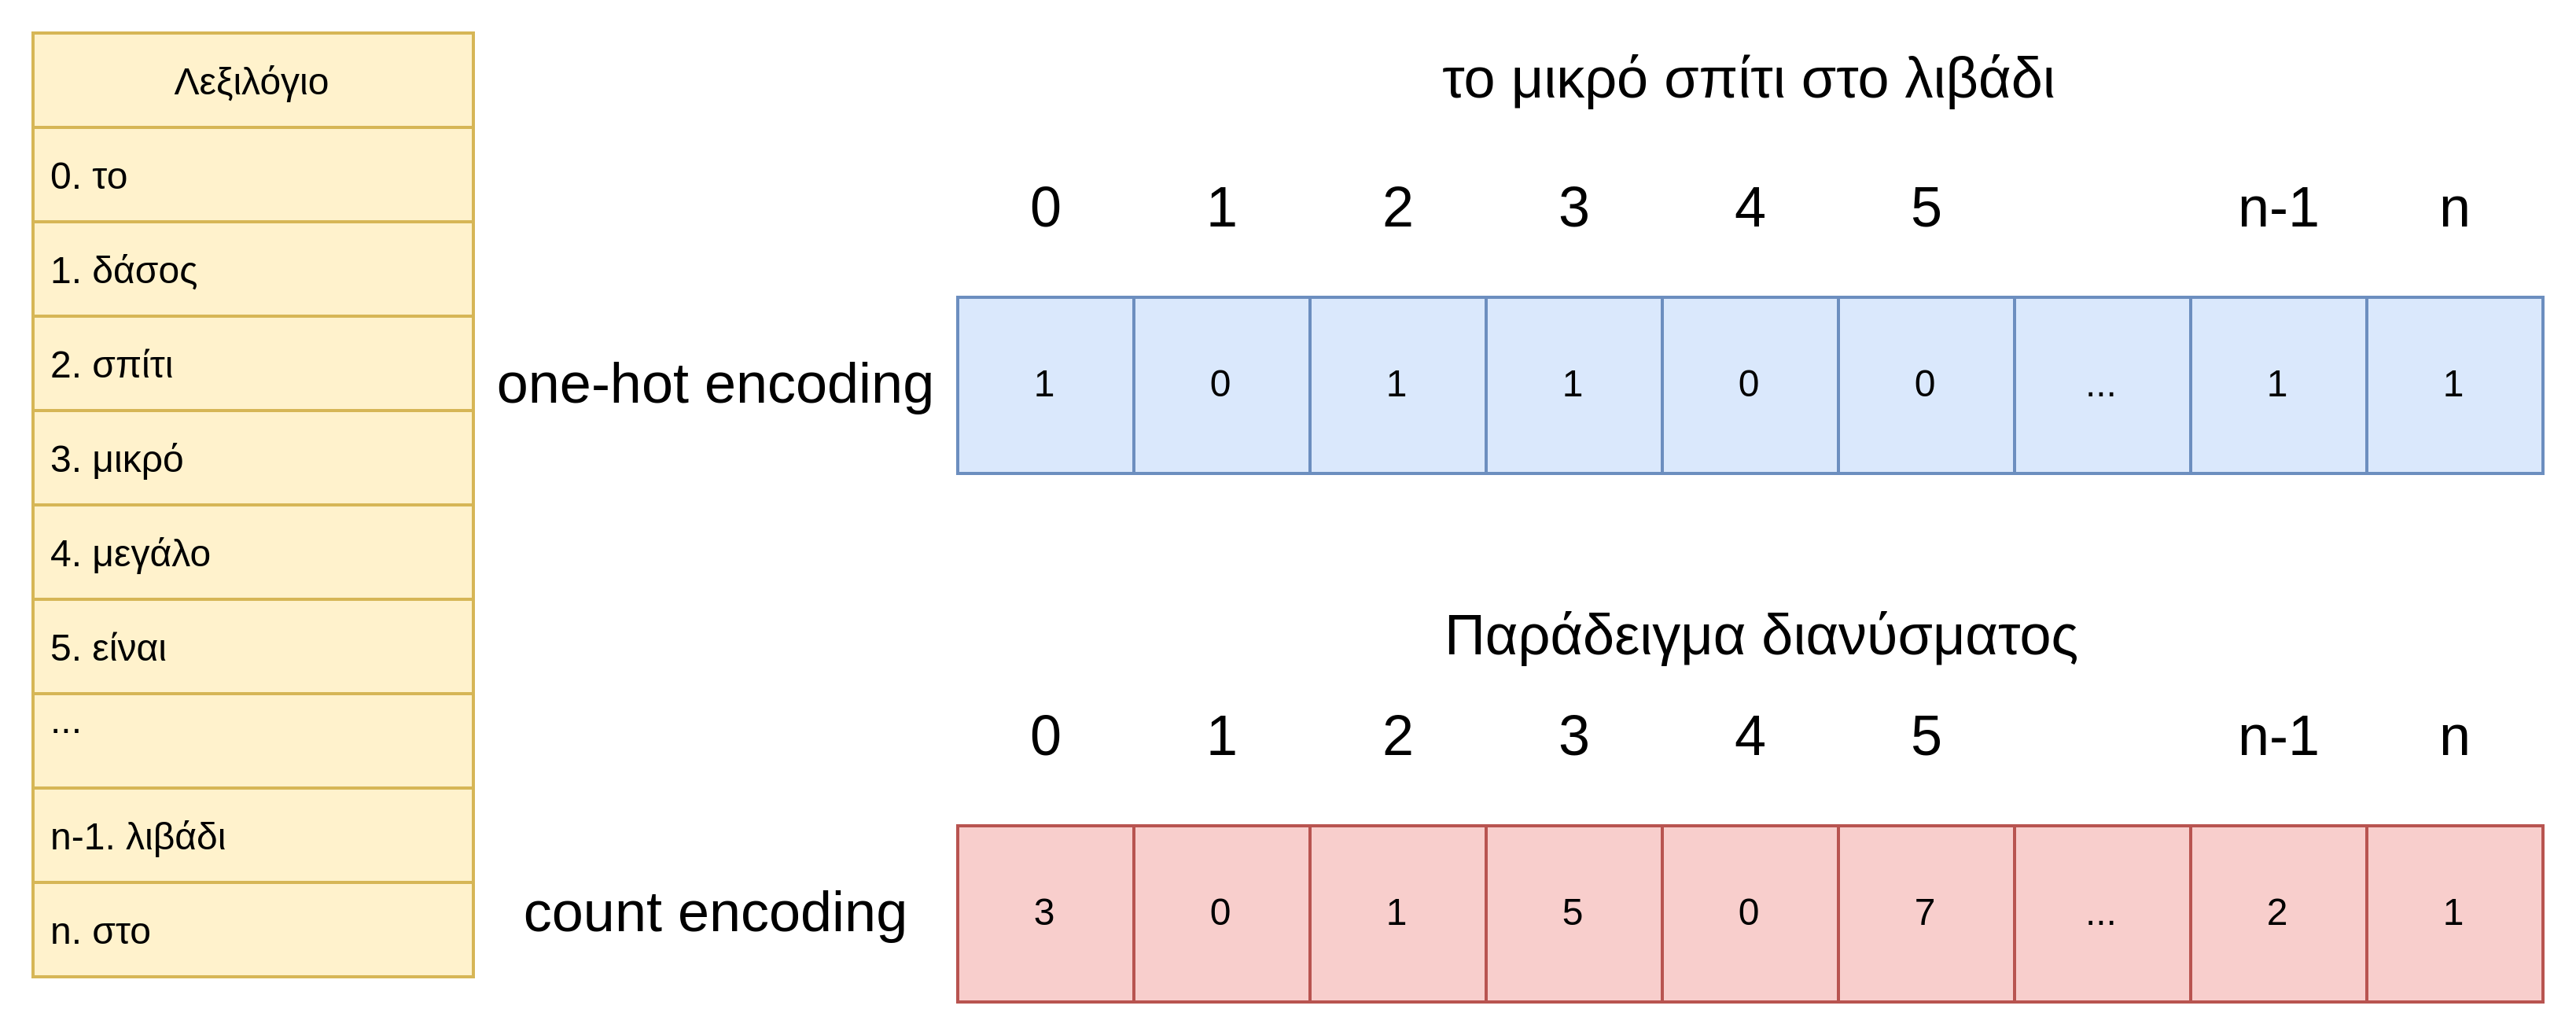
\includegraphics[width=0.7\textwidth]{images/chapter2/vector.png}
  \caption{Παράδειγμα διανυσμάτων \emph{one-hot encoding \& count encoding}}
  \label{fig:vector}
\end{figure}
\noindent

\subsection{Συχνότητα Εμφάνισης Όρου - Αντίστροφη Συχνότητα Εμφάνισης Εγγράφου}
Μία από τις πιο δημοφιλής τεχνικές δημιουργίας \emph{word embeddings} είναι η Συχνότητα Εμφάνισης Όρου - Αντίστροφη συχνότητα Εμφάνισης Εγγράφου (\emph{Term Frequency - Inverse Document Frequency - TF-IDF}). Αποτελεί μία στατιστική μέθοδο η οποία δείχνει πόσο σημαντική είναι μία λέξη σε ένα σύνολο από έγγραφα. Ο υπολογισμός της προκύπτει από το γινόμενο της συχνότητας εμφάνισης (\emph{Term Frequency - TF}) της λέξης στο αντίστοιχο έγγραφο, όπως και στο \emph{bag of words}, επί την αντίστροφη συχνότητα της λέξης σε όλα τα έγγραφα (\emph{Inverse Document Frequency - IDF}). Έστω ένα σύνολο από έγγραφα $D$ και έστω $t$ η λέξη της οποίας αναζητείται η \emph{TF-IDF} τότε:

\begin{equation}
    \label{eq:tfidf}
    \text{TF-IDF}(t,d) = TF \cdot \log {\frac{ |D| }{ 1 + | \{ f \in D : t \in f \} |}}
\end{equation}

όπου, στην \autoref{eq:tfidf}:

\begin{itemize}
    \item \emph{t}: η λέξη
    \item \emph{d}: το έγγραφο
    \item TF: το πλήθος των φορών που εμφανίζεται η λέξη στο αντίστοιχο έγγραφο
    \item |D|: ο συνολικός αριθμός των εγγράφων
    \item $| \{ f \in D : t \in f \} |$: το πλήθος των εγγράφων που εμφανίζεται η λέξη \emph{t}
\end{itemize}

Η μέθοδος \emph{TF-IDF} μπορεί επίσης να χρησιμοποιηθεί και για \emph{IR}. Έστω μια πρόταση της οποίας αναζητείται το πλησιέστερο έγγραφο. Για κάθε έγγραφο υπολογίζεται η μετρική \emph{TF-IDF} ως το άθροισμα των \emph{TF-IDF} κάθε λέξης στην πρόταση. Τα έγγραφα με τις μεγαλύτερες τιμές είναι και τα πιο πιθανά να σχετίζονται με την αρχική πρόταση.

\begin{equation}
    \label{eq:total-tfidf}
    \text{TF-IDF}(Q,d) = \sum_{t \in Q} TF \cdot \log {\frac{ |D| }{ 1 + | \{ f \in D : t \in f \} |}}
\end{equation}
όπου, στην \autoref{eq:total-tfidf}:
\begin{itemize}
    \item Q: η πρόταση
    \item t: μία λέξη της πρότασης
\end{itemize}

Παρά το γεγονός ότι η παραπάνω μέθοδος είναι αρκετά αποδοτική έχει δύο βασικά μειονεκτήματα. Όπως είναι εύκολα παρατηρήσιμο, όσο αυξάνεται η συχνότητα εμφάνισης της λέξης στο έγγραφο τόσο αυξάνεται και το σκορ της, χωρίς ωστόσο αυτό να σημαίνει ότι το συγκεκριμένο έγγραφο είναι πιο σχετικό με την αρχική πρόταση. Επιπλέον, η \emph{TF-IDF} δεν λαμβάνει καθόλου υπόψιν το μέγεθος του εγγράφου.

\subsection{\emph{BM25}}
Το σκορ \emph{BM25} είναι μία παραλλαγή του \emph{TF-IDF} που αναγνωρίζει τις αδυναμίες που αναφέρθηκαν παραπάνω και τις αντιμετωπίζει βασίζόμενο στην επιλογή δύο παραμέτρων. Η παράμετρος $k_1$ είναι υπεύθυνη για τον κορεσμό του \emph{TF} σε περίπτωση που κάποιος όρος εμφανίζεται πολλές φορές στο αντίστοιχο έγγραφο. Πιο συγκεκριμένα, το σκορ αυξάνεται γρήγορα στις αρχικές εμφανίσεις της λέξης στο κείμενο και σταδιακά επηρεάζει λιγότερο την άνοδο του σκορ. Επιπλέον, εισάγει την παράμετρο $b$ η οποία καθορίζει πόσο θα επηρεάζεται το σκορ από το μέγεθος του εγγράφου. Έτσι,προκύπτει η \autoref{eq:bm25}:

\begin{equation}
    \label{eq:bm25}
    \text{BM25}(Q,d) = \sum_{t \in Q} \frac{TF}{TF + k_1 \cdot (1 - b + b \cdot \frac{len_{doc}}{len_{avg}})} \cdot \log {\frac{|D| + 1}{| \{ f \in D : t \in f \} | + 0.5}}
\end{equation}

όπου:
\begin{itemize}
    \item Q: η πρόταση
    \item d: το αρχείο του οποίου το σκορ υπολογίζεται
    \item t: μία λέξη από την πρόταση Q
    \item TF: η συχνότητα εμφάνισης της λέξης στο έγγραφο d
    \item $len_{doc}$: το μέγεθος του εγγράφου d
    \item $len_{avg}$: ο μέσος όρος του μεγέθους όλων των εγγράφων
    \item |D|: ο συνολικός αριθμός των εγγράφων
    \item $| \{ f \in D : t \in f \} |$: το πλήθος των εγγράφων που εμφανίζεται η λέξη \emph{t}
\end{itemize}